\documentclass[10pt]{article}

\usepackage{akteach}
\usepackage{amsmath}
\usepackage{amsfonts}
\usepackage{amssymb}
\usepackage{amsthm}
\usepackage{float}
\usepackage{algpseudocode}
\usepackage[all]{xy}

\usepackage{listings}
\usepackage{color}

\definecolor{dkgreen}{rgb}{0,0.6,0}
\definecolor{gray}{rgb}{0.5,0.5,0.5}
\definecolor{mauve}{rgb}{0.58,0,0.82}

\lstset{
  language=Python,
  aboveskip=3mm,
  belowskip=3mm,
  showstringspaces=false,
  columns=flexible,
  basicstyle={\small\ttfamily},
  numbers=none,
  numberstyle=\tiny\color{gray},
  keywordstyle=\color{blue},
  commentstyle=\color{dkgreen},
  stringstyle=\color{mauve},
  breaklines=true,
  breakatwhitespace=true,
  tabsize=3
}


\newcommand{\C}{\mathbb{C}}
\newcommand{\Q}{\mathbb{Q}}
\newcommand{\K}{\mathbb{K}}
\newcommand{\proj}{\mathbb{P}}
\newcommand{\T}{\mathbb{T}}
\newcommand{\F}{\mathbb{F}}
\newcommand{\Z}{\mathbb{Z}}
\newcommand{\N}{\mathbb{N}}
\newcommand{\set}{\mathcal{S}}
\newcommand{\cp}{\mathbb{C}P}
\newcommand{\A}{\mathcal{A}}
\newcommand{\BB}{\mathcal{B}}
\newcommand{\CC}{\mathcal{C}}
\newcommand{\NN}{\mathcal{N}}
\newcommand{\LL}{\mathcal{L}}
\newcommand{\MM}{\mathcal{M}}
\newcommand{\E}{\mathcal{E}}
\newcommand{\FF}{\mathcal{F}}
\newcommand{\G}{\mathcal{G}}
\newcommand{\eps}{\varepsilon}
\newcommand{\Hom}{\text{Hom}}
\newcommand{\Div}{\text{div}}
\newcommand{\Res}{\text{Res}}
\newcommand{\ord}{\text{ord}}
\newcommand{\Deg}{\text{deg}}
\newcommand{\mult}{\text{mult}}

\newcommand{\id}{\text{id}}
\newcommand{\Tr}{\text{Tr}}
\newcommand{\ad}{\text{ad}}
\newcommand{\Ad}{\text{Ad}}
\newcommand{\Aut}{\text{Aut}}
\newcommand{\der}{\text{der}}
\newcommand{\GL}{\text{GL}}
\newcommand{\gl}{\mathfrak{gl}}
\newcommand{\rad}{\mathfrak{rad}}
\newcommand{\inhook}{\hookrightarrow}
\newcommand{\sgn}{\text{sign}}

\begin{document}

\akteachheader{Numerical Analysis (CS 450)}%
{4-Credit Hour Project, Bill Karr}

\akteachprobhead{%
  Part 1: Use Arnoldi to solve linear systems $\to$ GMRES
}

\begin{itemize}

\item[(a)] In the variant of the Arnoldi process shown in Algorithm 4.9 in the text, let $ Q_k $ be the matrix consisting of the first $k$ columns of $Q$, and let $ H_{k} $ be the top-left $(k+1) \times k$ submatrix of $H$. Show that after $q_{k+1}$ is added to $Q$ in the algorithm, at iteration $k$, the identity $ Q_{k+1}^T A Q_k = H_k $ holds. Does the `reverse' identity $ A = Q_{k+1} H_k Q_{k}^T $ hold as well?

\begin{proof}
From the line $ h_{jk} = q_j^T u_k = q_j^T A q_k $ for $ j = 1,2, ..., k $. If $ j = k+1 $, then the algorithm says that $$
q_{k+1} = \frac{1}{h_{k+1,k}} \left( Aq_k - \sum_{j = 1}^k h_{jk} q_j \right).
$$ Since $q_i$ are all unit vectors, then $$
 h_{k+1,k} = q_{k+1}^T \left( Aq_k - \sum_{j = 1}^k h_{jk} q_j \right) = 
 q_{k+1}^T Aq_k - \sum_{j = 1}^k h_{jk} q_{k+1}^T q_j .
$$ But since $ q_i $ are orthnormal, the terms in the sum vanish and this reduces to $ h_{k+1,k} =  q_{k+1}^T Aq_k.$ If $ i > j+1 $, then $h_{ij} = 0$ and $
q_{i}^T Aq_j = 0 $ because $ Aq_j \in \text{span} \{ q_0 , ... , q_{j+1} \} $ and $ q_i^T q_\ell = 0 $ for all $ \ell \leq j+1$.

We conclude that $ h_{ij} = q_i^T A q_j $ for all $ j \leq k, i \leq k+1 $. Thus, $ H_k = Q_{k+1}^T A Q_k $. 

The reverse identity does not hold generically since the rank of $ Q_{k+1} H_k Q_{k}^T $ is at most $ \text{rank}(Q_k) \leq k$ and the rank of $A$ could be larger.
\end{proof}

\item[(b)] If $ x_k \in K_k = \text{span} \{ b, ... , A^{k-1} b \} $ is the vector that minimizes the residual $ r_k = Ax_k - b $ in the 2-norm and $ x_k = Q_k y_k $, show that $ \| r_k \|_2 = \| H_k y_k - \| b \|_2 e_1 \|_2 $. 

\begin{proof}
First, by part (a), $ H_k y_k = Q_{k+1}^T A Q_k y_k = Q_{k+1}^T A x_k $. In addition, $ Q_{k+1}^T b = \| b \|_2 e_1 $ since the columns of $Q_k$ are orthogonal to $b$ except for the first one which is $b$ normalized. Thus, $$
\| H_k y_k - \| b \|_2 e_1 \|_2 = \| Q_{k+1}^T A x_k - Q_{k+1}^T b \|_2 = \| Q_{k+1}^T ( A x_k - b ) \|_2 = \| A x_k - b \|_2 = \| r_k \|_2 $$ since $ Q_{k+1} Q_{k+1}^T = I $.
\end{proof}

\item[(c)] Describe a procedure to find $x_k$, using a linear least-squares problem with $H_k$ as a building block. 

\begin{proof}[Solution]
Since $ x_k $ minimizes $ \| r_k \|_2 $, then if we can find $ y_k $ which minimizes $\| H_k y_k - \| b \|_2 e_1 \|_2 = \| r_k \|_2$, $x_k$ can be obtained by just multiplying $ Q_k $ to $y_k$. So, we solve the linear least squares problem $
H_k y_k \approx \| b \|_2 e_1 $ for $y_k$ and let $ x_k = Q_k y_k $.
\end{proof}

\newpage

\item[(d)] See \verb+my_gmres_d+ in \verb+gmres.py+ for my code. Here is my function:  \begin{lstlisting}
def my_gmres_d(A_func, b, tol=1e-10):
    """Solve Ax = b to an absolute residual norm of at most tol.

    Returns a tuple (x, num_iterations).

    Solution to Part 2(d) of the project assignment.
    """
    if la.norm(b) < tol:
        return 0 * b, 0
    if la.norm(A_func(b)) == 0:
        print "Warning: Krylov subspaces are trivial."
        return 0 * b, 0

    n = len(b)
    H = np.empty((1, 0))
    Q = np.empty((n, 1))
    Q[:, 0] = b / la.norm(b)
    x = b * np.dot(b, A_func(b)) / np.dot(A_func(b), A_func(b))
    y = np.empty((2, 1))
    vec = np.array([la.norm(b)])

    for k in xrange(n):
        print "performing iteration %d of GMRES..." % (k+1)
        H = np.column_stack((H, np.zeros(k + 1)))
        H = np.row_stack((H, np.zeros(k + 1)))
        u = A_func(Q[:, k])
        for j in xrange(k + 1):
            H[j, k] = np.dot(Q[:, j], u)
            u = u - H[j, k] * Q[:, j]
        H[k + 1, k] = la.norm(u)
        if H[k + 1, k] == 0:
            break
        Q = np.column_stack((Q, u / H[k + 1, k]))

        vec = np.append(vec, 0)
        y = la.lstsq(H, vec)[0]
        x = np.dot(Q[:, :-1], y)
        res = la.norm(b - A_func(x)) / la.norm(b)
        if res < tol:
            break

    if la.norm(b - A_func(x)) / la.norm(b) >= tol:
        print "Warning: tolerance was not met."
    return x, k + 1
\end{lstlisting}

Here's my output: \begin{verbatim}
----------------------------------------
part(d)
----------------------------------------
converged after 13 iterations
residual: 6.63889e-11
error: 8.8999e-10
\end{verbatim}

\newpage



\end{itemize}

\akteachprobhead{%
  Part 2: Derive an integral equation for a second-order boundary value problem
}

\begin{itemize}

\item[(a)] For any $ \varphi $, show that if $$
u(x) = \tau(x) u_a + (1 - \tau(x)) u_b + \frac{1}{L} \left( (b - x) \int_a^x \varphi(z) ( a - z ) \, dz +  (a - x) \int_x^b \varphi(z) ( b - z ) \, dz  \right),
$$ $ u(a) = u_a $ and $ u(b) = u_b $, where $ \tau(x) = 1 - (x-a)/L $, $ L = b - a $.

\begin{proof} Simply compute. $$
u(a) = \tau(a) u_a + (1 - \tau(a)) u_b + \frac{1}{L} \left( (b - a) \int_a^a \varphi(z) ( a - z ) \, dz +  (a - a) \int_a^b \varphi(z) ( b - z ) \, dz  \right)
$$ $$
= 1 \cdot u_a + 0 \cdot u_b + \frac{1}{L} \left( L \cdot 0 + 0 \cdot  \int_a^b \varphi(z) ( b - z ) \, dz \right) = u_a.
$$ Similarly, $$
u(b) = \tau(b) u_a + (1 - \tau(b)) u_b + \frac{1}{L} \left( (b - b) \int_a^b \varphi(z) ( a - z ) \, dz +  (a - b) \int_b^b \varphi(z) ( b - z ) \, dz  \right)
$$ $$
= 0 \cdot u_a + 1 \cdot u_b + \frac{1}{L} \left( 0 \cdot \int_a^b \varphi(z) ( a - z ) \, dz  - L \cdot 0 \right) = u_b.
$$
\end{proof}

\item[(b)] Show that $$
u'(x) = \frac{1}{L} \left( u_b - u_a - \int_a^x \varphi(z)(a - z) \, dz - \int_x^b  \varphi(z)(b - z) \, dz \right).
$$

\begin{proof} Using the fact that $ \tau'(x) = - \frac{1}{L} $ and the fundamental theorem of calculus combined with the chain rule, we obtain
$$
u'(x) = -\frac{u_a}{L} + \frac{u_b}{L} $$ $$+ \frac{1}{L} \left( 
(-1) \int_a^x \varphi(z) ( a - z ) \, dz + (b - x) \varphi(x) (a - x)
+ (-1) \int_x^b \varphi(z) ( b - z ) \, dz - (a - x) \varphi(x) (b - x)
 \right)
$$ $$
= \frac{1}{L}  \left( u_b - u_a - \int_a^x \varphi(z)(a - z) \, dz - \int_x^b  \varphi(z)(b - z) \, dz \right).
$$
\end{proof}

\item[(c)] Show that $ u''(x) = \varphi(x) $. 

\begin{proof}
Using the previous result, we again apply the fundamental theorem of calculus and obtain $$
u''(x) = \frac{1}{L} \left( - \varphi(x)(a - x) + \varphi(x)(b - x) \right) = \frac{\varphi(x) ( b - a )}{L} = \varphi(x).
$$
\end{proof}

\item[(d)] Show that if $ u $ satisfies $ u'' + p u' + q u = r  $, then $ \varphi $ satisfies the integral equation  $$
\varphi(x) + \int_{a}^b K(x,z) \varphi(z) \, dz = R(x)
$$ with the so-called `kernel'
 \begin{displaymath}
   K(x,z) = \left\{
     \begin{array}{lr}
       \frac{p(x) + (x - b)q(x)}{L} (z - a) & : z \leq x \\
       \frac{p(x) + (x - a)q(x)}{L} (z - b) & : z > x
     \end{array}
   \right.
\end{displaymath} and the right-hand side $$
R(x) = -\left( q(x)[ \tau(x) u_a + (1 - \tau(x)) u_b ] + \frac{p(x)}{L} ( u_b - u_a ) - r(x)  \right).
$$
\begin{proof}
Plugging $ u'', u', $ and $u$ into the differential equation, we obtain $$
u''(x) + p(x) u'(x) + q(x) u(x)  = \varphi(x) + \frac{p(x)}{L}  \left( u_b - u_a - \int_a^x \varphi(z)(a - z) \, dz - \int_x^b  \varphi(z)(b - z) \, dz \right) $$ $$ + q(x)\tau(x) u_a + q(x)(1 - \tau(x)) u_b + \frac{q(x)}{L} \left( (b - x) \int_a^x \varphi(z) ( a - z ) \, dz +  (a - x) \int_x^b \varphi(z) ( b - z ) \, dz  \right) $$ $$
= \varphi(x) + \int_a^x  \frac{p(x) + (x - b)q(x)}{L} (z - a) \varphi(x) \, dz
+ \int_x^b  \frac{p(x) + (x - a)q(x)}{L} (z - b) \varphi(x) \, dz
$$ $$
+ \left( q(x)[ \tau(x) u_a + (1 - \tau(x)) u_b ] + \frac{p(x)}{L} ( u_b - u_a )  \right)
$$ $$
= \varphi(x) + \int_a^b K(x,z) \varphi(z) \, dz + \left( q(x)[ \tau(x) u_a + (1 - \tau(x)) u_b ] + \frac{p(x)}{L} ( u_b - u_a )  \right) = r(x).
$$ Thus, moving the third summand to the right hand side, we obtain $$
\varphi(x) + \int_{a}^b K(x,z) \varphi(z) \, dz = R(x).
$$
\end{proof}
\end{itemize}

\newpage

\akteachprobhead{%
  Part 3: Build a BVP solver
}

\begin{itemize}

\item[(a)] See \verb+apply_kernel+ in \verb+bvp.py+. Here is my code:
\begin{lstlisting}
def apply_kernel(a, b, mesh, kernel, density):
    def trapz(f, mesh):
        return np.dot((f[1:] + f[:-1]) / 2, mesh[1:] - mesh[:-1])

    temp = np.zeros(len(mesh))
    for i in xrange(len(mesh)):
        left = trapz(kernel(mesh[i], mesh[:i + 1], -1) * density[:i + 1], mesh[:i + 1])
        right = trapz(kernel(mesh[i], mesh[i:], +1) * density[i:], mesh[i:])
        temp[i] = left + right
    return temp
\end{lstlisting}

\item[(b)] See \verb+solve_bvp+ in \verb+bvp.py+. Here is my code: \begin{lstlisting}
def solve_bvp(mesh, p, q, r, ua, ub):
    x = mesh
    a, b = mesh[0], mesh[-1]
    L = b - a

    def tau(x):
        return 1 - (x - a) / L

    def R(x):
        return -(q(x) * (tau(x) * ua + (1 - tau(x)) * ub) + p(x) * (ub - ua) / L - r(x))

    def K(x, z, sign):
        temp = np.empty(len(z))
        if sign == -1:
            temp[z <= x] = (p(x) + (x - b) * q(x)) * (z[z <= x] - a) / L
            temp[z > x] = (p(x) + (x - a) * q(x)) * (z[z > x] - b) / L
        if sign == +1:
            temp[z < x] = (p(x) + (x - b) * q(x)) * (z[z < x] - a) / L
            temp[z >= x] = (p(x) + (x - a) * q(x)) * (z[z >= x] - b) / L
        return temp

    def K2(x, z, sign):
        temp = np.empty(len(z))
        if sign == -1:
            temp[z <= x] = (x - b) * (z[z <= x] - a) / L
            temp[z > x] = (x - a) * (z[z > x] - b) / L
        if sign == +1:
            temp[z < x] = (x - b) * (z[z < x] - a) / L
            temp[z >= x] = (x - a) * (z[z >= x] - b) / L
        return temp

    def A_func(phi):
        return phi + apply_kernel(a, b, mesh, K, phi)

    phi, its = my_gmres_e(A_func, R(x))
    print "Solution found. For n = %d, GMRES took %g iteration(s)." % (len(x), its)
    print
    u = tau(x) * ua + (1 - tau(x)) * ub + apply_kernel(a, b, mesh, K2, phi)
    return u

\end{lstlisting}

\newpage

\item[(c)] See \verb+bvp.py+ for my code. Here is the output upon running \verb+test_bvp.py+.

\begin{verbatim}
h=0.0301003 err=0.270672
h=0.003001 err=0.00268591
test_poisson: EOC: 2.00074

h=0.0301003 err=0.426333
h=0.003001 err=0.00386274
test_with_p: EOC: 2.04019

h=0.0301003 err=2.07232
h=0.003001 err=0.0187981
test_with_q: EOC: 2.03968

h=0.0301003 err=0.332962
h=0.003001 err=0.00303815
test_full_enchilada: EOC: 2.03713
\end{verbatim}

\item[(d)] See \verb+test_bvp.py+ for my code. I observe that the number of iterations it takes for GMRES to solve does not depend on the number of subintervals for each test. The test with $q$ only shows up for one size $n$ because it takes 8 iterations for both the test with $p$ and the test with $q$. Here is my plot: 

\begin{figure}[H]
  \centering
    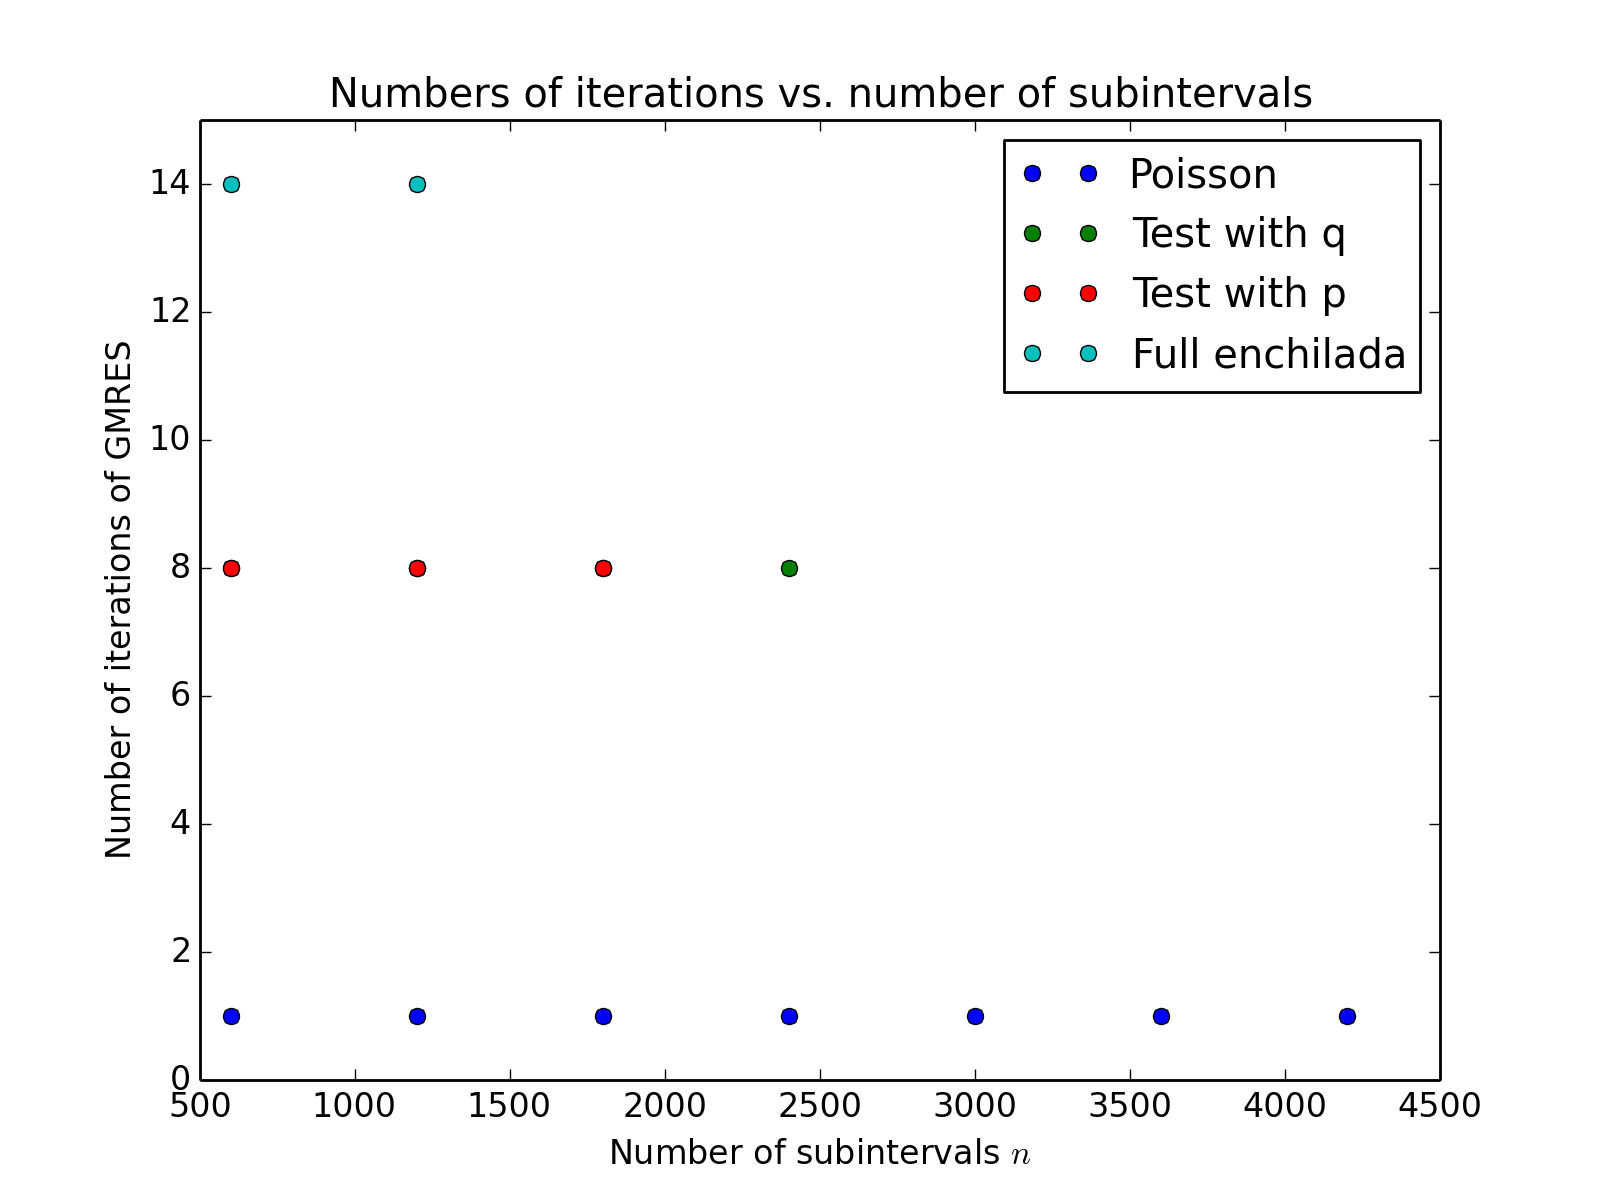
\includegraphics[scale=0.63]{iteration_counts}
\end{figure}

\end{itemize}

\newpage

\akteachprobhead{%
  Part 4: A toolkit for composite high-order discretization
}

\begin{itemize}

\item[(a)] See \verb+__init__+ in \verb+legendre_discr.py+. Here is my code: \begin{lstlisting}
def __init__(self, intervals, order):
    self.intervals = intervals
    self.nintervals = len(intervals) - 1
    self.npoints = order + 1
    self.mid_pts = (self.intervals[1:] + self.intervals[:-1]) / 2
    self.scales = (self.intervals[1:] - self.intervals[:-1]) / 2
    self.sample_nodes = sp.legendre(self.npoints).weights[:, 0].real
    self.sample_weights = sp.legendre(self.npoints).weights[:, 1].real
    # taking real part because sometimes sp.legendre is returning
    # complex numbers with zero imaginary part and displaying a warning

    nodes = (self.mid_pts + np.outer(self.sample_nodes, self.scales)).T
    self.nodes = np.reshape(nodes, -1)
    weights = np.outer(self.scales, self.sample_weights)
    self.weights = np.reshape(weights, -1)

    monos = np.array([self.sample_nodes ** k for k in range(self.npoints)])
    integrals = np.array([(self.sample_nodes ** (k + 1) - (-1) ** (k + 1)) / (k + 1)
                         for k in range(self.npoints)])
    self.spec_int_mat = la.solve(monos, integrals)
\end{lstlisting}

\item[(b)] See \verb+integral+ in \verb+legendre_discr.py+. Here is my code: \begin{lstlisting}
def integral(self, f):
    return np.dot(f, self.weights)
\end{lstlisting}

\item[(c)] See \verb+left_indefinite_integral+ and \verb+right_indefinite_integral+ in \verb+legendre_discr.py+. Here is my code: \begin{lstlisting}
def left_indefinite_integral(self, f):
    d = self.npoints
    n = self.nintervals
    f = f.reshape((n, d))
    weights = self.weights.reshape((n, d))
    integrals = np.cumsum(np.einsum('ij,ij->i', f, weights))
    integrals = np.roll(integrals, 1)
    integrals[0] = 0
    indef = np.dot((f.T * self.scales).T, self.spec_int_mat)
    indef = (integrals + indef.T).T
    indef = np.reshape(indef, -1)
    return indef

def right_indefinite_integral(self, f):
    return self.integral(f) - self.left_indefinite_integral(f)
\end{lstlisting}

\newpage

\item[(d)] Upon running \verb+test_legendre_discr.py+, here is the output.

\begin{verbatim}
---------------------------------
ORDER 2
---------------------------------
h=0.1 err=0.118027
h=0.0333333 err=0.00168249
<lambda>: EOC: 3.8691

h=0.1 err=0.141862
h=0.0333333 err=0.0016825
<lambda>: EOC: 4.03652

---------------------------------
ORDER 3
---------------------------------
h=0.1 err=0.0455367
h=0.0333333 err=0.000125478
<lambda>: EOC: 5.36508

h=0.1 err=0.0456416
h=0.0333333 err=0.000125478
<lambda>: EOC: 5.36718

---------------------------------
ORDER 5
---------------------------------
h=0.1 err=0.00221849
h=0.0333333 err=5.46588e-07
<lambda>: EOC: 7.56285

h=0.1 err=0.00221849
h=0.0333333 err=5.46588e-07
<lambda>: EOC: 7.56285

---------------------------------
ORDER 7
---------------------------------
h=0.1 err=6.48553e-05
h=0.0333333 err=1.47309e-09
<lambda>: EOC: 9.73278

h=0.1 err=6.48553e-05
h=0.0333333 err=1.47309e-09
<lambda>: EOC: 9.73278
\end{verbatim}

\end{itemize}

\newpage

\akteachprobhead{%
  Part 5: Build a fast and accurate BVP solver
}

\begin{itemize}

\item[(a)] See \verb+fast_bvp.py+. The code for my \verb+apply_kernel+ function is: \begin{lstlisting}
def apply_kernel(discr, fl, gl, fr, gr, density):
    """
    :arg discr: an instance of
        :class:`legendre_discr.CompositeLegendreDiscretization`
    :arg fl,gl,fr,gr: functions of a single argument
    """
    x = discr.nodes
    Gl = discr.left_indefinite_integral(gl(x) * density)
    Gr = discr.right_indefinite_integral(gr(x) * density)
    result = fl(x) * Gl + fr(x) * Gr
    return result
\end{lstlisting}

\item[(b)] See \verb+fast_bvp.py+. The code for my \verb+solve_bvp+ function is:\begin{lstlisting}
def solve_bvp(discr, p, q, r, ua, ub):
    """
    :arg discr: an instance of
        :class:`legendre_discr.CompositeLegendreDiscretization`
    """
    a, b = discr.intervals[0], discr.intervals[-1]
    L = b - a

    def tau(x):
        return 1 - (x - a) / L

    def R(x):
        return -(q(x) * (tau(x) * ua + (1 - tau(x)) * ub) + p(x) * (ub - ua) / L - r(x))

    def fl(x):
        return (p(x) + (x - b) * q(x)) / L

    def fr(x):
        return (p(x) + (x - a) * q(x)) / L

    def gl(x):
        return x - a

    def gr(x):
        return x - b

    def fl2(x):
        return (x - b) / L

    def fr2(x):
        return (x - a) / L

    def A_func(phi):
        return phi + apply_kernel(discr, fl, gl, fr, gr, phi)

    x = discr.nodes
    phi, its = my_gmres_e(A_func, R(x))
    u = tau(x) * ua + (1 - tau(x)) * ub + apply_kernel(discr, fl2, gl, fr2, gr, phi)

    return u
\end{lstlisting}

\item[(c)] Upon running \verb+test_fast_bvp.py+, my output was: \begin{verbatim}
----------------------------------------------
test_poisson -- order 3
----------------------------------------------
h=0.02 err=0.00426799
h=0.01 err=0.000129103
get_error: EOC: 5.04697

----------------------------------------------
test_poisson -- order 5
----------------------------------------------
h=0.02 err=8.76324e-06
h=0.01 err=6.4139e-08
get_error: EOC: 7.09412

----------------------------------------------
test_poisson -- order 7
----------------------------------------------
h=0.02 err=9.53116e-09
h=0.01 err=1.69574e-11
get_error: EOC: 9.13459

----------------------------------------------
test_with_p -- order 3
----------------------------------------------
h=0.02 err=1.41895
h=0.01 err=0.0745256
get_error: EOC: 4.25095

----------------------------------------------
test_with_p -- order 5
----------------------------------------------
h=0.02 err=0.203782
h=0.01 err=0.00295016
get_error: EOC: 6.11008

----------------------------------------------
test_with_p -- order 7
----------------------------------------------
h=0.02 err=0.018239
h=0.01 err=6.41014e-05
get_error: EOC: 8.15245

----------------------------------------------
test_with_q -- order 3
----------------------------------------------
h=0.02 err=3.6688
h=0.01 err=0.0760487
get_error: EOC: 5.59224

----------------------------------------------
test_with_q -- order 5
----------------------------------------------
h=0.02 err=0.204061
h=0.01 err=0.00295022
get_error: EOC: 6.11203

----------------------------------------------
test_with_q -- order 7
----------------------------------------------
h=0.02 err=0.0182281
h=0.01 err=6.41023e-05
get_error: EOC: 8.15157

----------------------------------------------
test_full_enchilada -- order 3
----------------------------------------------
h=0.02 err=1.43841
h=0.01 err=0.0744792
get_error: EOC: 4.2715

----------------------------------------------
test_full_enchilada -- order 5
----------------------------------------------
h=0.02 err=0.203789
h=0.01 err=0.00295022
get_error: EOC: 6.11011

----------------------------------------------
test_full_enchilada -- order 7
----------------------------------------------
h=0.02 err=0.0182401
h=0.01 err=6.41023e-05
get_error: EOC: 8.15252
\end{verbatim}

\newpage

\item[(d)] Each time GMRES runs, my code outputs the number of iterations. It appears that for a fixed test, the number of iterations it takes to converge does not depend on the matrix size. Here is my plot:

\begin{figure}[H]
  \centering
    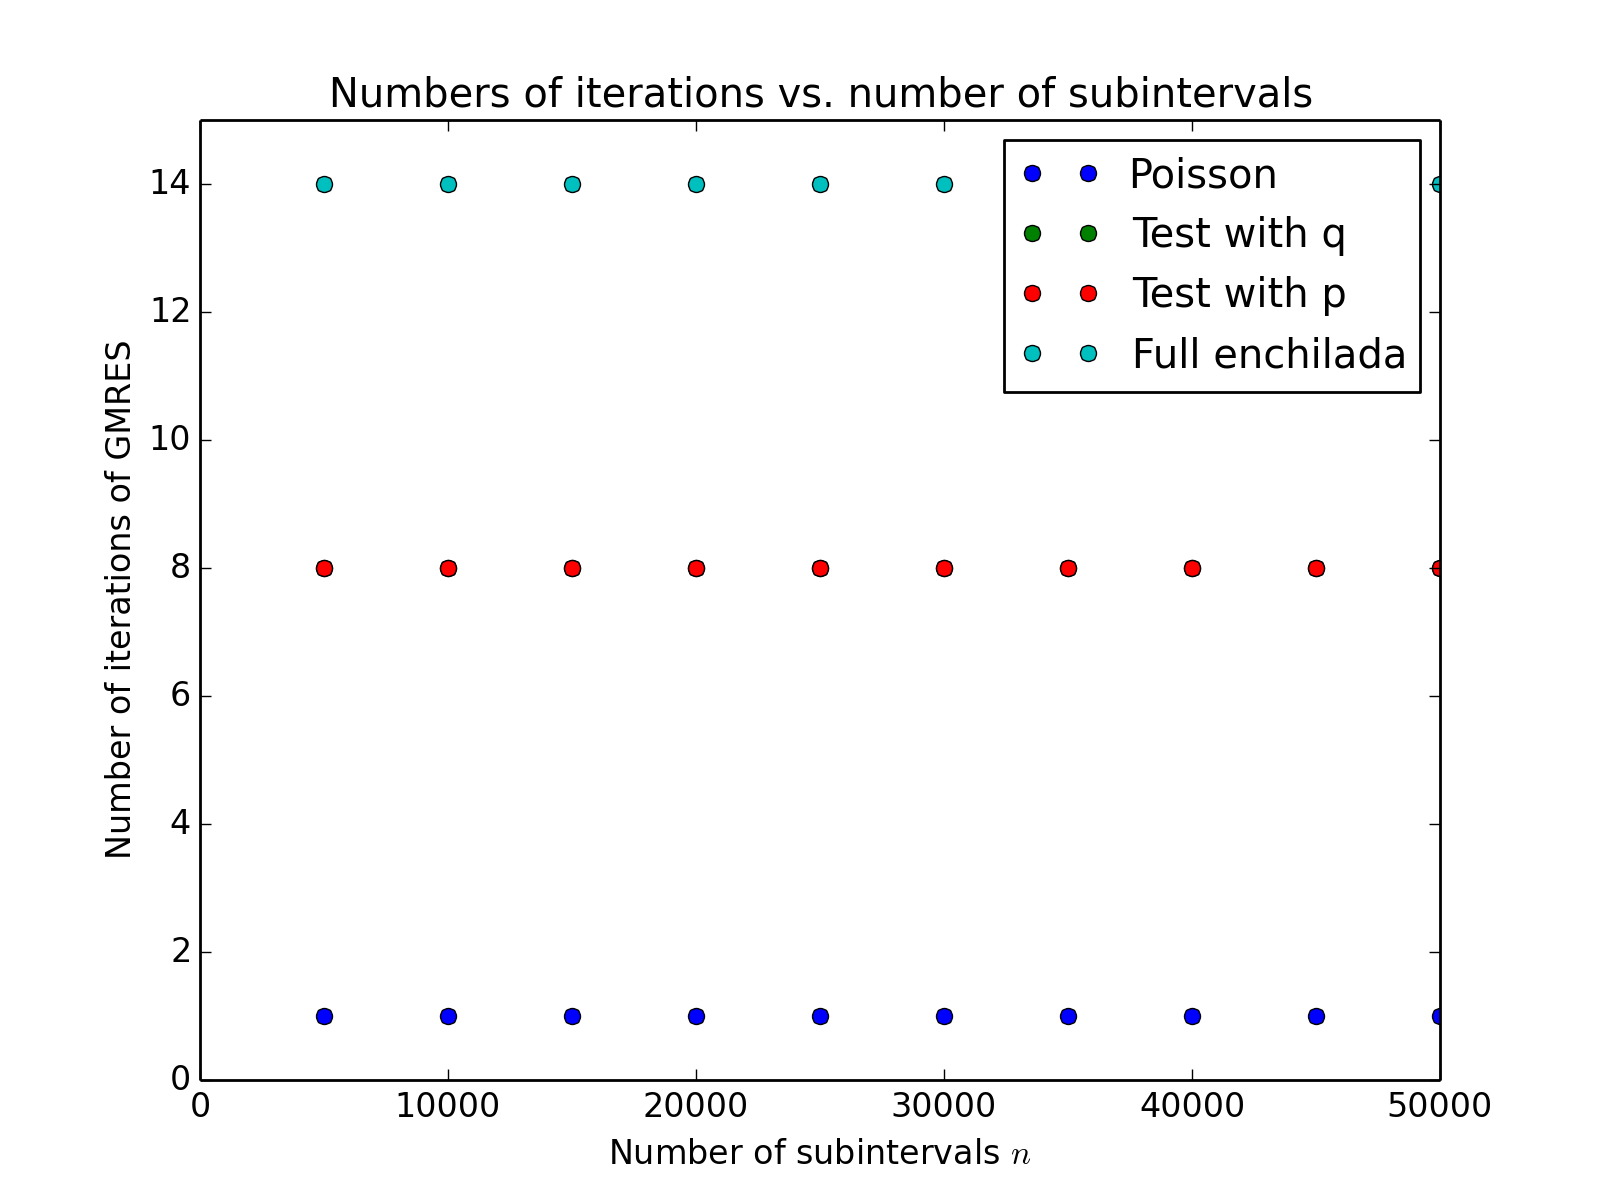
\includegraphics[scale=0.63]{fast_iteration_counts}
\end{figure}

\item[(e)] See \verb+timing.py+ for my code. Here is a graph of my results for numbers of subintervals $ n = 2^9, ..., 2^{20} $. After finding the best fit linear relationship between $ \log(t) $ and $ \log(n) $ I obtain $ t \propto n^{1.04489} $, so the algorithm runs in approximately linear time.

\begin{figure}[H]
  \centering
    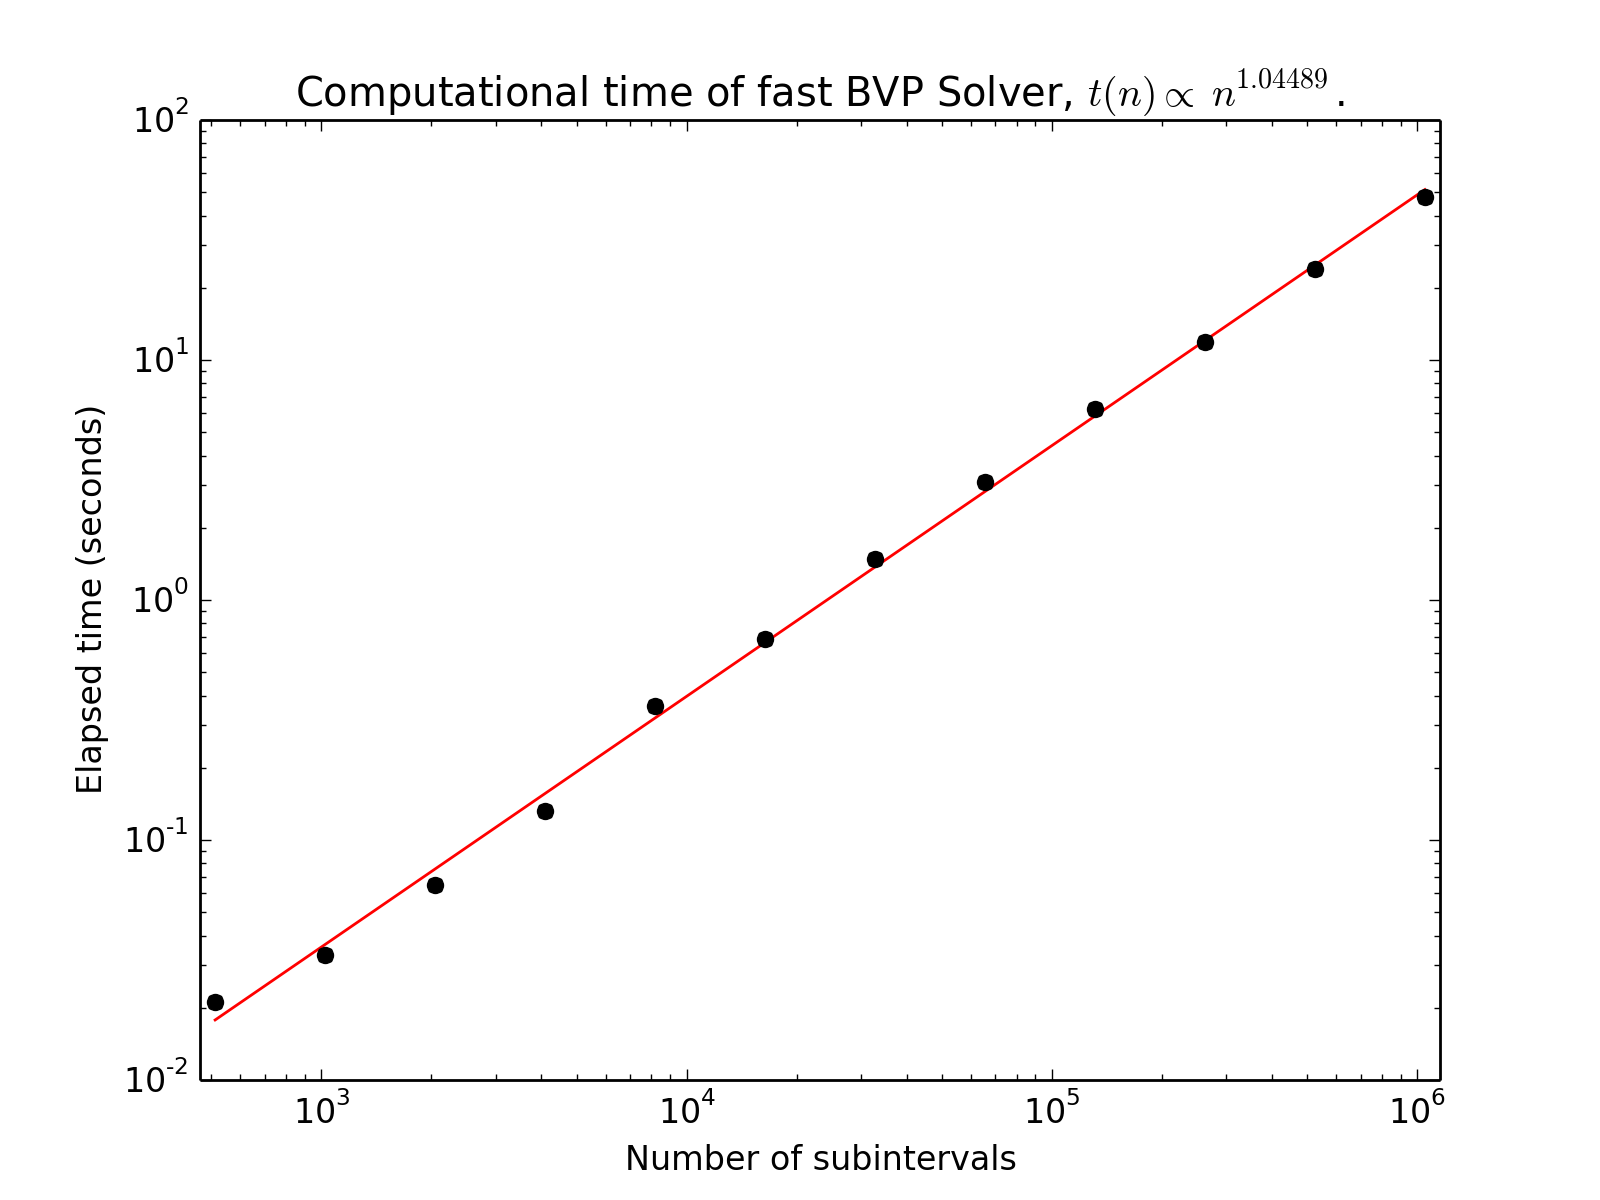
\includegraphics[scale=0.63]{timing}
\end{figure}

\end{itemize}

\end{document}
